\section{Aufgabenstellung}

Bei diesem Experiment soll die Verbrennungsenthalpie $\Delta _C U$ einer unbekannten Substanz, mit einem Bombenkalorimeter nach Berthelot, bestimmt werden.


\section{Durchführung}



\begin{table}[H]
	\centering
	\begin{tabular}{llc}
		\toprule
		Messung & Substanz    & Einwaage[g] \\
		\midrule
		1       & Benzoesäure & 0.512       \\
		2       & Substanz M  & 0.545       \\
		3       & Substanz M  & 0.555g      \\
		4       & Benzoesäure & 0.576       \\
		\bottomrule
	\end{tabular}
	\caption{Gewichte der Tabletten}
\end{table}

Die bekannten Werte sind:
\begin{itemize}
    \item $M[Benz.] = 122.12 g/mol$
    \item das Molekulargewicht der unbekannten Substanz M $M[M] = 152 g/mol$
    \item der Brennwert des Zünddrahts: $30 J$
    \item der Brennwert des Baumwollfadens: $50 J$
    \item die Verbrennungsenthalpie von der Benzoesäure $\Delta _C U = -3226 \, KJ/mol$
\end{itemize}

\section{Versuchsaufbau}

\begin{figure}[H]
    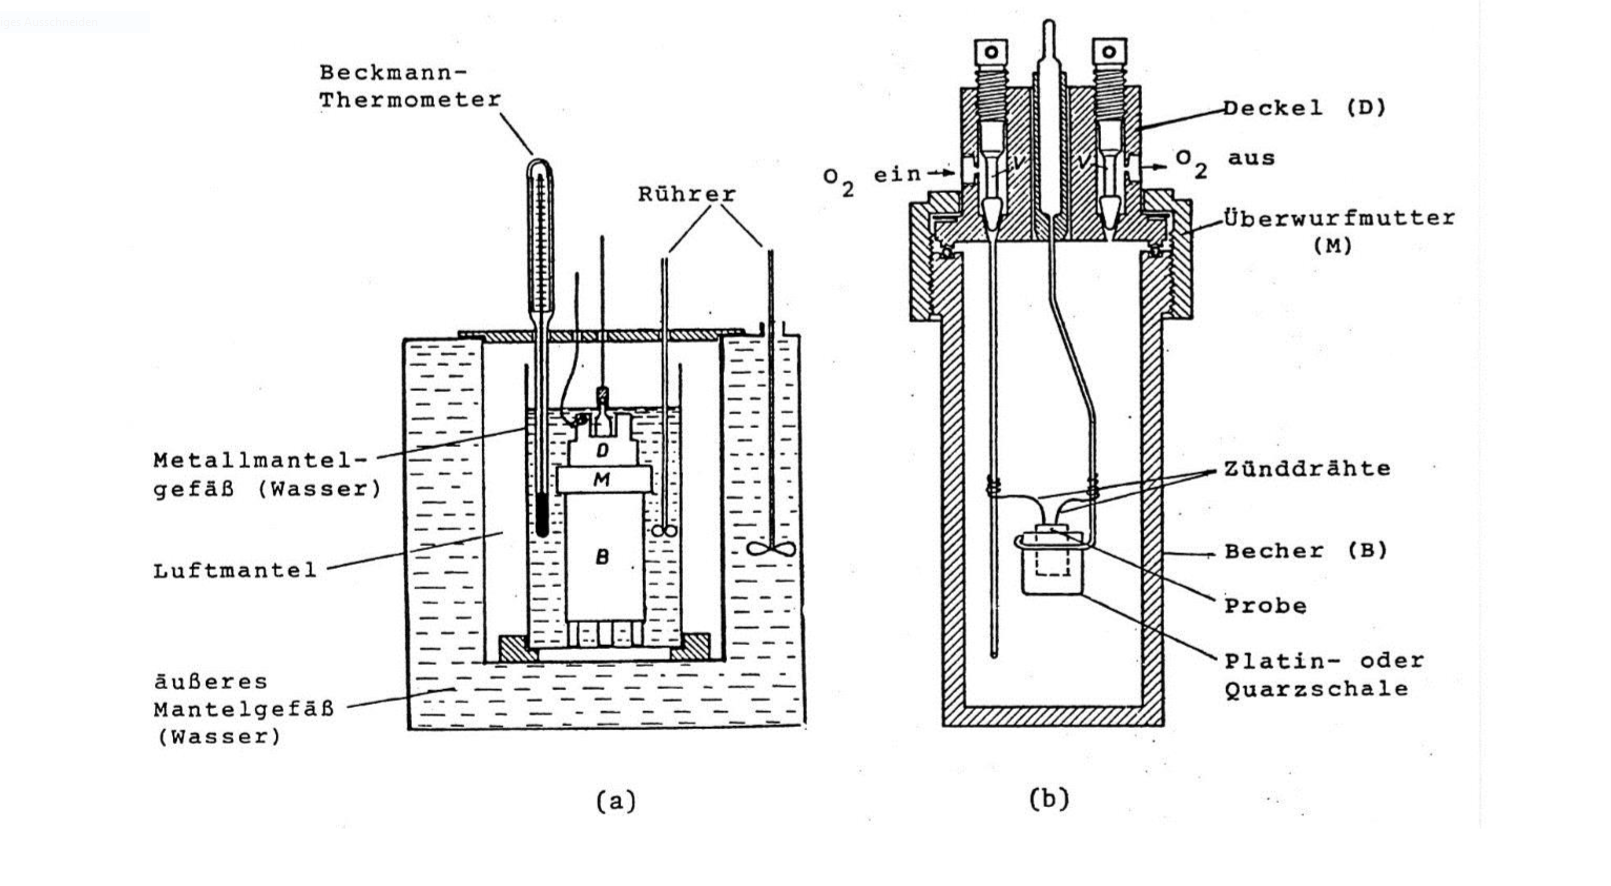
\includegraphics[width=\linewidth]{C:/Users/josefk/Desktop/kalorimetrie/src/img/bombenkalorimeter.PNG}
    \caption{Aufbau eines Bombenkalorimeters}
\end{figure}




